\documentclass[11pt]{article}
\usepackage[T1]{fontenc}
\usepackage{lmodern}
\usepackage[a4paper,margin=2.5cm]{geometry}
\usepackage{amsmath,amssymb,amsthm}
\usepackage{booktabs}
\usepackage{graphicx}
\usepackage[font=small,labelfont=bf]{caption}
\usepackage{microtype}
\usepackage[hidelinks]{hyperref}
\hypersetup{pdftitle={Access to Cash after ATM Consolidation in Luxembourg},pdfauthor={Eugenio Guilarte Homayden}}
\usepackage{setspace}
\usepackage[authoryear,round]{natbib}
\setstretch{1.08}
\setlength{\parskip}{0.35em}
\newtheorem{proposition}{Proposition}

\title{Access to Cash after ATM Consolidation in Luxembourg:\\ Road Distances, Bounds on Lost Access, and Machine Placement}
\author{Eugenio Guilarte Homayden\thanks{University of Macerata. E-mail: \texttt{euge.guilarte@gmail.com}. Code, data, and results: \url{https://github.com/GeneTheStoic/cash-access-luxembourg}. Prepared in November 2026 as a preliminary analysis for an application to a doctoral position on cash infrastructures, to understand the problem and test one possible research direction with open data.}}
\date{Preliminary analysis, November 2026}

\begin{document}
\maketitle

\begin{abstract}
\noindent Luxembourg's five largest retail banks are replacing their separate ATM fleets with one shared network, Bancomat. This note measures what the change means for residents' access to cash, using only open data: the 2021 census population on the 1\,km grid, the public Bancomat locator (214 machines at 207 sites), ATM locations recovered from OpenStreetMap at four dates, and road distances computed on the national road network. Three results follow. First, 92.8\% of residents will live within 5\,km by road of a Bancomat machine, which reproduces the operator's figure of about 92\%; the mean road distance is 1.82\,km, against 1.2\,km reported for Austria. Second, because the open record of the old networks is incomplete, the comparison with January 2024 yields lower bounds on lost access: at least 14,601 residents will be more than 2\,km farther from cash, and at least 10,807 will move beyond 5\,km. Third, 13 additional machines placed by a greedy coverage rule would raise coverage within 5\,km to 97.1\%, against 94\% for the 13 sites the operator has identified. The note ends with the questions that bank and central bank data would answer.
\end{abstract}

\section{Introduction}
In 2026 the banks BGL BNP Paribas, BIL, Banque Raiffeisen, POST Luxembourg, and Spuerkeess began replacing their ATM fleets with a shared network operated by LuxConstellation under the Bancomat brand. The network will have about 237 machines, against 595 cash machines in 2019; the operator expects 92\% of the population to be within 5\,km by road of a machine, and 13 further sites under study would raise this to 94\% \citep{paperjam2026}. Installation proceeds at four to eight machines per week until 2027, and the legacy Spuerkeess network is to be decommissioned in summer 2027 \citep{spuerkeess2026}.

Central banks follow access to cash because it conditions who can still pay in cash and how a digital euro would be adopted. The Oesterreichische Nationalbank measured road distances to ATMs for the whole Austrian population \citep{stix2020}; the Bank of Canada measured access for First Nations reserves \citep{chen2021}; the Banque de France publishes yearly accessibility reports \citep{bdf2025}. For Luxembourg, the Banque centrale du Luxembourg estimates that 22\% of consumers prefer cash and 1\% use only cash \citep{giordana2026}. This note adds a measurement of the consolidation itself, with three contributions: an independent reproduction of the operator's coverage figure; bounds on the number of residents who lose access, which remain valid although the record of the old networks is incomplete; and a placement analysis that shows where additional machines would raise coverage most.

\section{Data}
\emph{Population.} STATEC's 2021 census on the 1\,km INSPIRE grid (EPSG:3035) gives 643,420 residents in 1,636 populated cells; each cell is assigned to the commune covering most of its area. The share of residents aged 65 and over is available by commune (1 January 2018) and is applied to the cells of each commune.

\emph{Bancomat network.} The public locator lists 214 machines at 207 distinct sites, of which 22 were in service on 5 November 2026. The operator notes that the map is indicative and that some sites are still to be confirmed.

\emph{Legacy networks.} ATMs and banks tagged with an ATM were recovered from OpenStreetMap at four dates (July 2019, January 2024, June 2026, and November 2026) through historical queries, kept only inside the national boundary, and merged when closer than 30\,m. The January 2024 record has 283 mapped objects at 246 sites, which is well below the 595 machines reported for 2019: the open record is incomplete, and Section~\ref{sec:bounds} shows how to use it anyway.

\emph{Roads.} The drivable OpenStreetMap network of Luxembourg, with a 2--3\,km margin, has 29,340 nodes and 37,206 links after simplification \citep{boeing2017}.

\section{Method}
Each cell is represented by its centroid and each site by its coordinates, both snapped to the nearest road node (median snap distance 278\,m for cells). The road distance from a cell to the nearest machine of a network is computed with one multi-source Dijkstra search from a virtual node linked to all site nodes, with link weights equal to the snap distances; the code is checked against brute force on synthetic road grids. Road distances are on average 1.41 times the straight-line distance for residents more than 1\,km from a machine. All shares are weighted by residents.

\subsection{Bounds on lost access}\label{sec:bounds}
Let $d^{\mathrm{true}}_i$ be the road distance from cell $i$ to the nearest legacy machine and $d^{\mathrm{OSM}}_i$ the distance computed from the mapped subset. If every mapped ATM existed, the mapped set is a subset of the true set, so $d^{\mathrm{true}}_i \le d^{\mathrm{OSM}}_i$ for every cell.

\begin{proposition}
Let $d^{\mathrm{B}}_i$ be the distance to the nearest Bancomat machine. For any threshold $c \ge 0$, the number of residents whose distance increases by more than $c$, and the number who move beyond any radius $R$, computed from the mapped legacy network, are lower bounds of the true numbers. The number of residents who move closer is an upper bound.
\end{proposition}

\noindent\emph{Proof.} $d^{\mathrm{B}}_i - d^{\mathrm{true}}_i \ge d^{\mathrm{B}}_i - d^{\mathrm{OSM}}_i$, so every cell with $d^{\mathrm{B}}_i - d^{\mathrm{OSM}}_i > c$ also satisfies the inequality for the true network; and $d^{\mathrm{OSM}}_i \le R$ implies $d^{\mathrm{true}}_i \le R$. The converse statement for cells moving closer follows from the same inequality. \qed

\subsection{Placement}
Two classical location problems are solved greedily over candidate sites at the populated cells, using the cell-to-cell road distance matrix. The maximal covering problem \citep{church1974} adds machines one at a time to maximize the residents newly within 5\,km; because coverage is a monotone submodular function, the greedy choice attains at least $1-1/e$ of the optimal gain for any number of additions \citep{nemhauser1978}. The $p$-median problem \citep{hakimi1964} places the same number of sites as the Bancomat plan to minimize the mean distance of residents. Both objectives count residents only; commuters, shoppers, and tourists are outside the model.

\section{Results}
\begin{table}[t]
\centering\small
\caption{Road distance from residents to the nearest ATM site.}
\label{tab:coverage}
\begin{tabular}{lrrrrrrr}
\toprule
Network & Sites & Mean & Median & P90 & $\le$1\,km & $\le$5\,km & Beyond 5\,km \\
 & & (km) & (km) & (km) & (\%) & (\%) & (residents) \\
\midrule
Bancomat plan (Nov 2026) & 207 & 1.82 & 1.14 & 4.42 & 42.6 & 92.8 & 46,073 \\
OSM, July 2019 & 210 & 2.07 & 1.22 & 5.56 & 40.9 & 87.7 & 79,057 \\
OSM, January 2024 & 246 & 1.93 & 1.16 & 4.95 & 43.0 & 90.1 & 63,497 \\
OSM, June 2026 & 225 & 2.02 & 1.17 & 5.27 & 43.3 & 88.9 & 71,110 \\
\bottomrule
\end{tabular}
\par\smallskip\footnotesize OSM rows describe the mapped part of the legacy networks only, which is incomplete.
\end{table}

\emph{The operator's figure is reproduced.} With the 207 planned sites, 92.8\% of residents live within 5\,km by road of a machine (Table~\ref{tab:coverage}), close to the 92\% announced by the operator; the median resident is 1.14\,km away and 72.1\% are within 2\,km. Access is less dense than in Austria, where the mean road distance is 1.2\,km, 82\% of residents are within 2\,km, and 2.9\% are beyond 5\,km \citep{stix2020}; in Luxembourg 7.2\% of residents, 46,073 people, are beyond 5\,km. The gap between small and large communes is also wider: residents of communes with fewer than 2,000 inhabitants are on average 4.61\,km from a machine, against 1.66\,km elsewhere (in Austria, 2.1\,km in municipalities below 2,000 inhabitants and 0.6\,km in larger cities). The residents with the longest distances are in the north and center-west (Figure~\ref{fig:maps}): in Kiischpelt, Putscheid, Bourscheid, and Grosbous, the mean road distance exceeds 7\,km.

\emph{Lost access, as lower bounds.} Compared with the mapped network of January 2024, at least 66,361 residents will be more than 0.5\,km farther from cash, at least 30,185 more than 1\,km farther, and at least 14,601 more than 2\,km farther; at least 10,807 residents move from within 5\,km to beyond it. The largest increases are in Saeul (+4.6\,km on average), Sandweiler (+3.6\,km), Kehlen (+2.4\,km), Putscheid, Lintgen, and Helperknapp (Figure~\ref{fig:maps}, right). Some of these communes may receive one of the sites the operator has not yet confirmed. The commune share of residents aged 65 and over is not associated with larger increases (weighted correlation $-0.07$), and the share of older residents within 5\,km (93.5\%) is close to that of all residents; this check uses commune averages and cannot see differences within communes.

\begin{figure}[t]
\centering
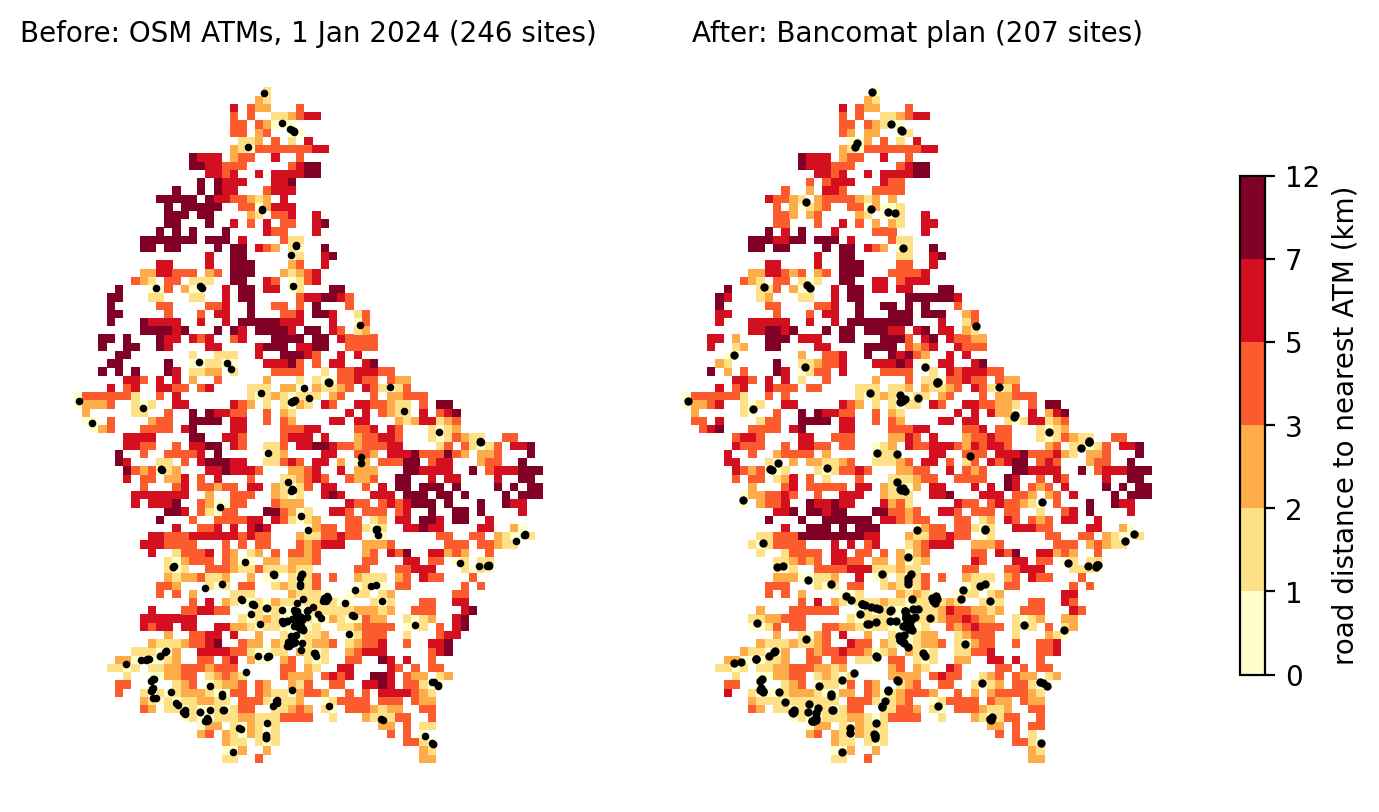
\includegraphics[width=0.66\textwidth]{../figures/map_distance.png}\hfill
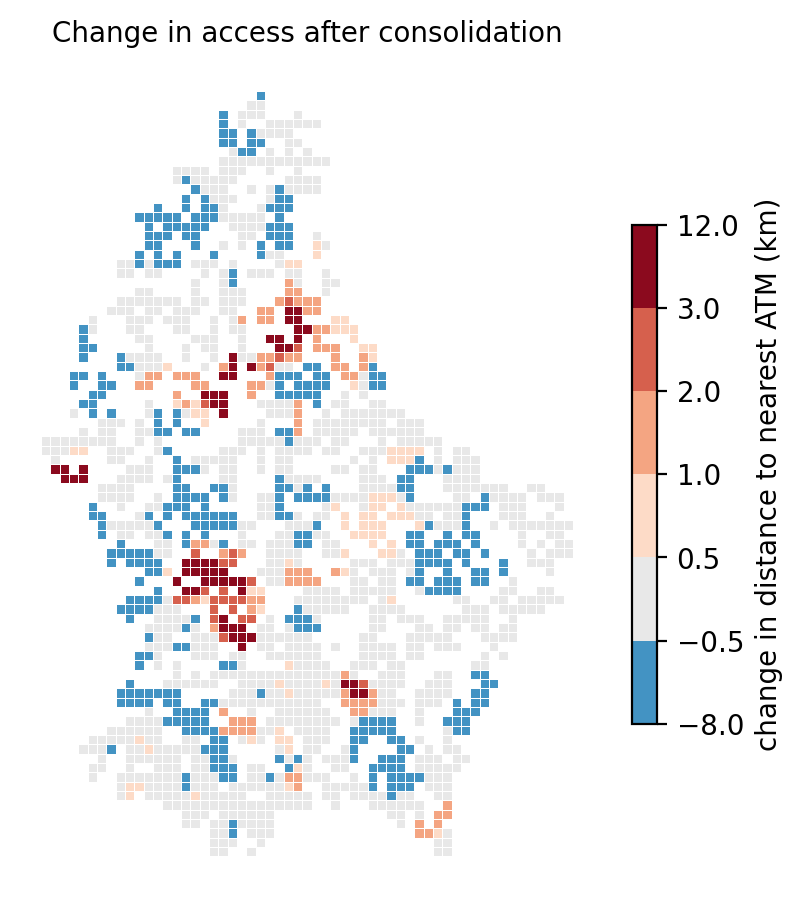
\includegraphics[width=0.33\textwidth]{../figures/map_change.png}
\caption{Left and center: road distance from each populated 1\,km cell to the nearest mapped legacy ATM (January 2024) and to the nearest planned Bancomat site. Right: change in distance; increases are lower bounds (Proposition 1).}
\label{fig:maps}
\end{figure}

\emph{Placement.} Thirteen machines added by the greedy covering rule raise coverage within 5\,km from 92.8\% to 97.1\%, about twice the gain the operator reports for its 13 candidate sites (Figure~\ref{fig:greedy}); the first three additions fall in Helperknapp, Grosbous, and Contern. With the same 207 sites placed to minimize the mean distance of residents, the mean would fall from 1.82 to 0.85\,km and coverage within 5\,km would reach 99.3\%. The comparison does not show that the plan is inefficient: for 39 of the 207 planned sites no resident has that site as the nearest one (straight-line catchments), because several machines are placed close together in the capital and in commercial centers, where people work and shop. The distribution of residents across the catchment areas of the sites is very unequal (Gini coefficient 0.51). A placement that serves residents and a placement that serves daytime demand differ, and the data needed to weigh them belong to the banks and the central bank.

\begin{figure}[t]
\centering
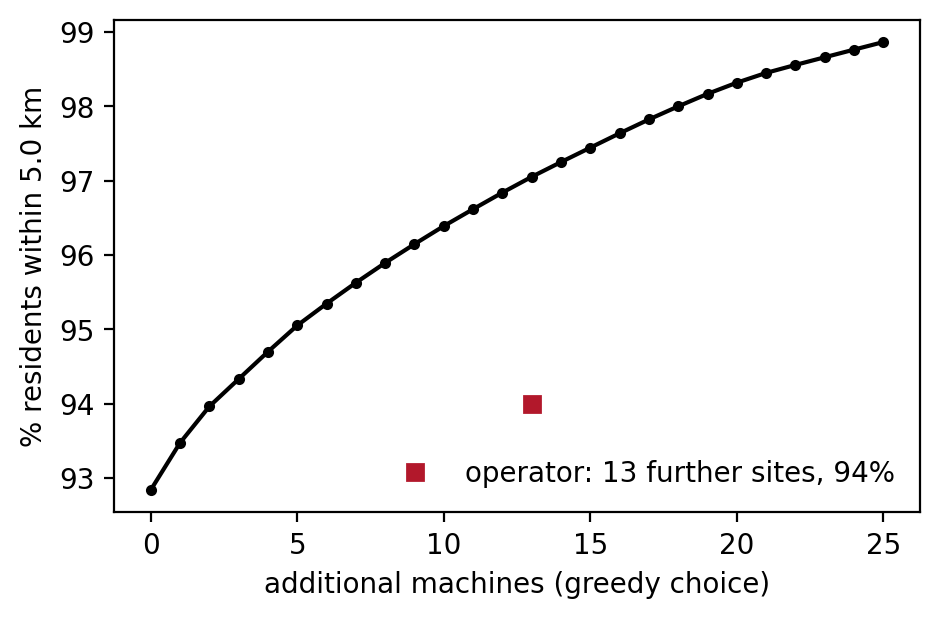
\includegraphics[width=0.48\textwidth]{../figures/greedy_additions.png}\hfill
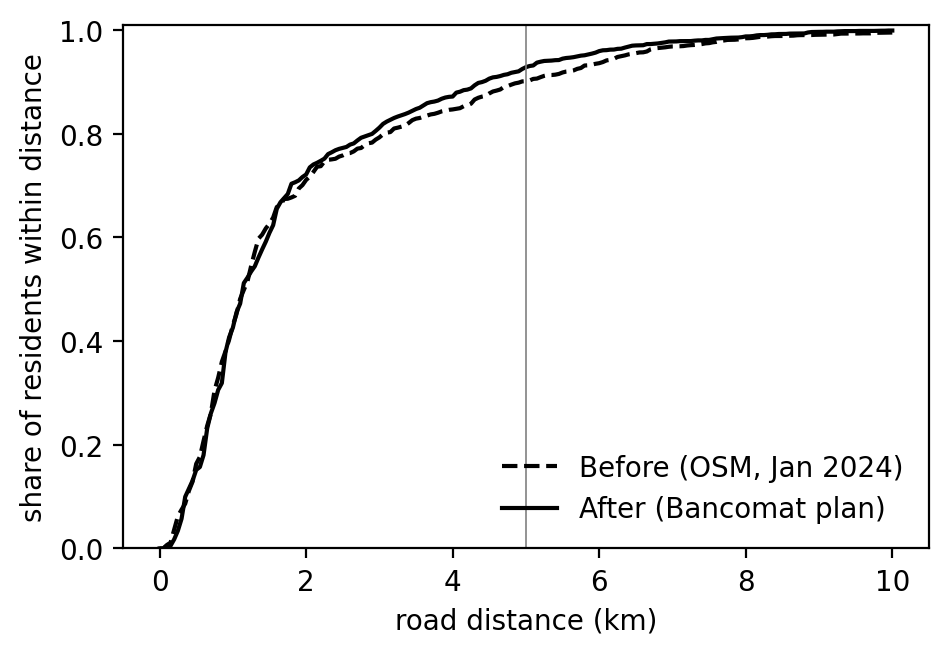
\includegraphics[width=0.48\textwidth]{../figures/coverage_curves.png}
\caption{Left: coverage within 5\,km by road as machines are added by the greedy covering rule, with the operator's figure for its 13 candidate sites. Right: share of residents within each road distance, mapped legacy network (January 2024) and Bancomat plan.}
\label{fig:greedy}
\end{figure}

\section{What bank and central bank data would add}
The rollout replaces machines place by place over about a year, which makes it a staggered natural experiment. With withdrawals by machine and payment data by area, the change in distance measured here becomes a treatment of varying intensity, and estimators for staggered adoption \citep{callaway2021} can identify how cash use responds to distance, separately for older residents, small communes, and cross-border commuters. That response is the missing parameter in two decisions: the placement problem above, where it would weight residents by the cash they actually withdraw, and the forecasts of digital euro adoption, where cash-preferring consumers who lose a nearby machine may shift to cards or to a digital wallet \citep{giordana2026}. Daytime population and card transaction data would also allow the placement to be evaluated against the demand the operator designs for.

\paragraph{Limitations.} The Bancomat map is indicative. The legacy record is incomplete, so changes are reported as bounds. Distances run from cell centroids, so residents of the same cell share one distance. Age is measured at commune level and is from 2018.

\paragraph{Reproducibility.} All data are public. Downloading the OpenStreetMap data and computing road distances took about 20 minutes on a laptop; the analysis then runs in about ten seconds and gave identical results on two machines.

\paragraph{Use of AI tools.} Claude (Anthropic) was used as an assistant for the Python implementation.

\begin{thebibliography}{99}
\bibitem[Boeing(2017)]{boeing2017} Boeing, G. (2017). OSMnx: New methods for acquiring, constructing, analyzing, and visualizing complex street networks. \emph{Computers, Environment and Urban Systems}, 65, 126--139.
\bibitem[Banque de France(2026)]{bdf2025} Banque de France (2026). \emph{Public access to cash in metropolitan France: update report, year-end 2025}.
\bibitem[Callaway and Sant'Anna(2021)]{callaway2021} Callaway, B. and Sant'Anna, P. H. C. (2021). Difference-in-differences with multiple time periods. \emph{Journal of Econometrics}, 225(2), 200--230.
\bibitem[Chen et al.(2021)]{chen2021} Chen, H., Engert, W., Huynh, K., and O'Habib, D. (2021). An exploration of First Nations reserves and access to cash. Bank of Canada Staff Discussion Paper 2021-8.
\bibitem[Church and ReVelle(1974)]{church1974} Church, R. and ReVelle, C. (1974). The maximal covering location problem. \emph{Papers of the Regional Science Association}, 32, 101--118.
\bibitem[Giordana(2026)]{giordana2026} Giordana, G. (2026). Assessing consumer CBDC adoption in Luxembourg: A micro-simulation approach. \emph{Journal of Financial Services Research}, 70(1). Earlier version: BCL Working Paper 193 (2025).
\bibitem[Hakimi(1964)]{hakimi1964} Hakimi, S. L. (1964). Optimum locations of switching centers and the absolute centers and medians of a graph. \emph{Operations Research}, 12(3), 450--459.
\bibitem[Nemhauser et al.(1978)]{nemhauser1978} Nemhauser, G. L., Wolsey, L. A., and Fisher, M. L. (1978). An analysis of approximations for maximizing submodular set functions, I. \emph{Mathematical Programming}, 14, 265--294.
\bibitem[Paperjam(2026)]{paperjam2026} Paperjam (2026). Bancomat: \texteuro70m for the last 200 cash machines. \url{https://en.paperjam.lu/article/bancomat-eu70m-for-the-last-200-cash-machines}.
\bibitem[Spuerkeess(2026)]{spuerkeess2026} Spuerkeess (2026). Bancomat: Luxembourg's new ATM network. \url{https://www.spuerkeess.lu/en/bancomat/}.
\bibitem[Stix(2020)]{stix2020} Stix, H. (2020). A spatial analysis of access to ATMs in Austria. \emph{Monetary Policy \& the Economy}, Q3/20, 39--59. Oesterreichische Nationalbank.
\end{thebibliography}
\end{document}
